\documentclass[12pt,a4paper, hidelinks]{article}
\usepackage[utf8]{inputenc}
\usepackage{amsmath}
\usepackage{amsfonts}
\usepackage{amssymb}
\usepackage{amsthm}
\usepackage{graphicx}
\usepackage{hyperref}
\usepackage{geometry}
\geometry{a4paper, margin=1in}
\usepackage{fancyhdr}
\usepackage{indentfirst} % Add this line to enable first paragraph indentation
\usepackage{times} % Use Times New Roman font
\usepackage{setspace}
\usepackage{graphicx}
\usepackage{float}
\usepackage{listings}

\setstretch{1.15} % Adjust the stretch factor as needed

\pagestyle{fancy}
\fancyhf{}  % Clear header and footer fields
\rfoot{\thepage}  % Place page number at the right bottom corner
\renewcommand{\headrulewidth}{0pt}  % Remove the header line


\begin{document}

\section*{SKaMP. Tests}
\addcontentsline{toc}{section}{Introduction}
\vspace{\baselineskip} % Add an empty line after the section title

The goal of this report is to provide information on the performed testing of data acquisition and data pre-processing.

GitHub repository: \href{https://github.com/salveendutt/Big-Data-Analytics}{https://github.com/salveendutt/Big-Data-Analytics}.

\section{Data acquisition}

\begin{table}[htbp]
\centering
\begin{tabular}{|p{3cm}|p{4cm}|p{4cm}|p{5cm}|}
\hline
\textbf{Test objective} & \textbf{Steps} & \textbf{Expected Result} & \textbf{Actual Result} \\
\hline
Verify data incoming from stream API & 1. Start the server using start\_containers.bat; 2. Navigate to http://localhost:5000 & Incoming data is stored in the file & TBD: screenshot \\
\hline
\end{tabular}
\caption{Data acquisition tests}
\end{table}

\section{Data pre-processing}

TBD

\begin{table}[htbp]
\centering
\begin{tabular}{|p{3cm}|p{4cm}|p{4cm}|p{5cm}|}
\hline
\textbf{Test objective} & \textbf{Steps} & \textbf{Expected Result} & \textbf{Actual Result} \\
\hline
Verify correct data pre-processing of dataset 1 & Run 'pytest' from the root folder & Incoming data is stored in the file & TBD: screenshot \\
\hline
\end{tabular}
\caption{Data pre-processing tests}
\end{table}

\begin{figure}[htbp]
  \centering
  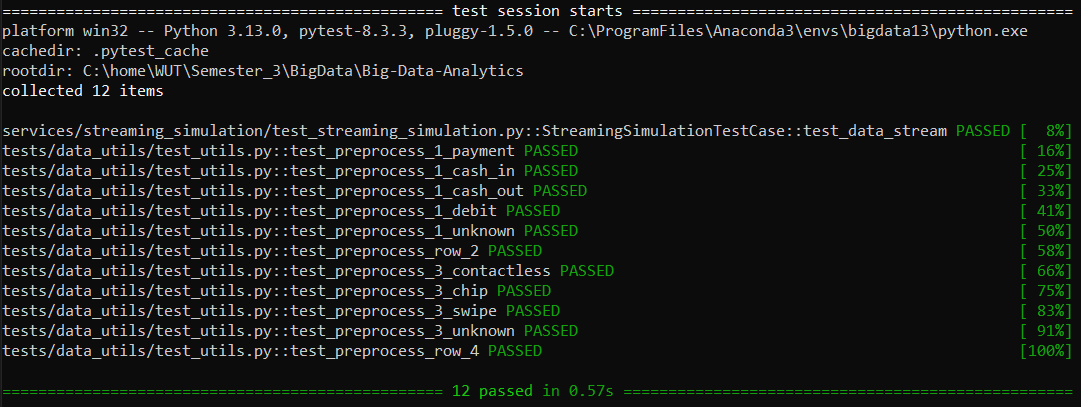
\includegraphics[width=0.95\textwidth]{images/unittests-M2.png}
  \caption{Unit testing result}
  \label{fig:sunset}
\end{figure}

Unit testing is included in the CI pipeline on GitHub and must be successful before any merge into the main branch.



\end{document}